\documentclass[tcc,capa]{texufpel}

\usepackage[utf8]{inputenc} % acentuacao
\usepackage{graphicx} % para inserir figuras
\usepackage[T1]{fontenc}
\usepackage{hyperref}
\hypersetup{
    hidelinks, % Remove coloração e caixas
    unicode=true,   %Permite acentuação no bookmark
    linktoc=all %Habilita link no nome e página do sumário
}

\unidade{Centro de Desenvolvimento Tecnológico}
\curso{Engenharia de Computação}
\nomecurso{Bacharelado em Engenharia de Computação}
\titulocurso{Bacharel em Engenharia de Computação}

\unidadeeng{Technology Development Center}
\cursoeng{Computer Science}


\title{VideoLearnAI: LLM Powered Web Application para aprendizagem ativa com vídeos do Youtube}

\author{Weitgenant}{Kevin Castro}
\advisor[Prof.~Dr.]{Primo}{Tiago}
\coadvisor[Prof.~Dr.]{Aguiar}{Marilton Sanchotene de}

%Palavras-chave em PT_BR
%use letras minúsculas seguidas por ;
%a última terminada por .
\keyword{palavrachave-um;}
\keyword{palavrachave-dois;}
\keyword{palavrachave-tres;}
\keyword{palavrachave-quatro.}

%Palavras-chave em EN_US
\keywordeng{keyword-one;}
\keywordeng{keyword-two;}
\keywordeng{keyword-three;}
\keywordeng{keyword-four.}

\begin{document}

%\renewcommand{\advisorname}{Orientadora}           %descomente caso tenhas orientadora
%\renewcommand{\coadvisorname}{Coorientadora}      %descomente caso tenhas coorientadora

\maketitle 

\sloppy

\fichacatalografica

%\folhadeaprovacao

%Composição da Banca Examinadora
\begin{aprovacao}{16 de março de 2025} %data da banca por extenso
\noindent Prof. Dr. Marilton Sanchotene de Aguiar (orientador)\\
Doutor em Computação pela Universidade Federal do Rio Grande do Sul.\\[1cm]

\noindent Prof. Dr. Paulo Roberto Ferreira Jr.\\
Doutor em Computação pela Universidade Federal do Rio Grande do Sul.\\[1cm]

\noindent Prof. Dr. Ricardo Matsumura Araujo\\
Doutor em Computação pela Universidade Federal do Rio Grande do Sul.\\[1cm]

\noindent Prof. Dr. Luciano da Silva Pinto\\
Doutor em Biotecnologia pela Universidade Federal de Pelotas.
\end{aprovacao}

%Opcional
\begin{dedicatoria}
  Dedico\ldots 
\end{dedicatoria}

%Opcional
\begin{agradecimentos}
  Agradeço\ldots 
\end{agradecimentos}

%Opcional
\begin{epigrafe}
  Só sei que nada sei.\\
  {\sc --- Sócrates}
\end{epigrafe}

%Resumo em Portugues (no maximo 500 palavras)
\begin{abstract}
  Este trabalho apresenta o desenvolvimento de uma plataforma educacional como serviço (SaaS) que utiliza Inteligência Artificial para aprimorar a experiência de aprendizagem com conteúdo em vídeo. O sistema implementa cinco funcionalidades principais: melhoria automática da legibilidade de legendas, geração de capítulos, transcrição sincronizada, geração de quizzes interativos e um sistema de bate-papo contextual com o conteúdo do vídeo. A solução emprega Large Language Models (LLMs) e arquitetura Transformer para processar e transformar o conteúdo audiovisual em material educacional interativo. A implementação foi realizada com foco em escalabilidade e performance, utilizando processamento em GPU e técnicas modernas de desenvolvimento de software. Os resultados demonstram o potencial da plataforma para transformar vídeos em experiências de aprendizagem mais engajadoras e efetivas.
  
  \end{abstract}
  
  %Resumo em Inglês (no maximo 500 palavras)
  \begin{englishabstract}{AI-Powered Educational Platform: Transforming Video Content into Interactive Learning Experiences}
  This work presents the development of an educational Software as a Service (SaaS) platform that leverages Artificial Intelligence to enhance video-based learning experiences. The system implements five main functionalities: automatic subtitle readability improvement, chapter generation, synchronized transcription, interactive quiz generation, and a contextual chat system for video content. The solution employs Large Language Models (LLMs) and Transformer architecture to process and transform audiovisual content into interactive educational material. The implementation focused on scalability and performance, utilizing GPU processing and modern software development techniques. The results demonstrate the platform's potential for transforming videos into more engaging and effective learning experiences.
  
  \end{englishabstract}

%Lista de Figuras
\listoffigures

%Lista de Tabelas
\listoftables

%lista de abreviaturas e siglas
\begin{listofabbrv}{ABNT}%coloque aqui a maior sigla para ajustar a distância
        \item[ABNT] Associação Brasileira de Normas Técnicas
        \item[NUMA] Non-Uniform Memory Access
        \item[SIMD] Single Instruction Multiple Data
        \item[SMP] Symmetric Multi-Processor
        \item[SPMD] Single Program Multiple Data
\end{listofabbrv}

%Sumario
\tableofcontents

\chapter{Introdução}
Nos últimos anos, o consumo de conteúdo educacional em vídeo tem crescido exponencialmente, impulsionado por plataformas como YouTube, Coursera e Udemy. Hoje, é possível encontrar aulas completas de universidades de altíssimo nível, como MIT, Harvard e Stanford, gratuitamente disponíveis online. No entanto, apesar da abundância de material de qualidade, muitos usuários enfrentam dificuldades em absorver e reter conhecimento de forma eficiente. A maioria das pessoas consome esses conteúdos de maneira passiva, apenas assistindo aos vídeos sem um envolvimento ativo com o material. Isso limita a retenção e a compreensão das informações.

A aprendizagem ativa, por outro lado, é um modelo comprovadamente mais eficaz, pois envolve o estudante em processos como resumo, questionamento, reorganização do conteúdo e interação com o material. Pesquisas mostram que métodos ativos de estudo, como fazer perguntas sobre o conteúdo, testar-se frequentemente e organizar a informação de forma estruturada, levam a um aprendizado mais profundo e duradouro. 

Diante desse cenário, este trabalho apresenta o desenvolvimento de um Software as a Service (SaaS) voltado para transformar o consumo passivo de vídeos educacionais em um processo de aprendizagem ativa. A solução utiliza modelos de linguagem natural (LLMs) para reestruturar legendas em textos mais legíveis, gerar capítulos automáticos, fornecer resumos e permitir interações como perguntas e respostas sobre o conteúdo. Além disso, o sistema oferece quizzes dinâmicos para reforçar o aprendizado e um mecanismo para salvar o progresso dos usuários, incentivando um envolvimento mais estruturado com os vídeos.

O desenvolvimento do SaaS seguiu uma abordagem iterativa. A arquitetura da aplicação integra tecnologias como FastAPI, Next.js e Transformers, além de estratégias de otimização para garantir eficiência e escalabilidade. A validação da ferramenta inclui métricas de desempenho e feedback dos usuários, avaliando sua eficácia na melhoria da compreensão e retenção do conhecimento.

Com esta pesquisa, buscamos não apenas oferecer uma ferramenta inovadora para aprendizado com vídeos, mas também contribuir para a democratização da educação de qualidade, permitindo que qualquer pessoa tenha acesso a um método mais eficaz para extrair o máximo de conhecimento dos conteúdos disponíveis online.

\section{Objetivo geral}
O objetivo geral deste trabalho é desenvolver um Software as a Service (SaaS) que transforme o consumo passivo de vídeos educacionais em um processo de aprendizagem ativa. Para isso, a plataforma utilizará inteligência artificial para melhorar a legibilidade das legendas, gerar resumos, estruturar conteúdos em capítulos, criar quizzes interativos e permitir interações diretas com o conteúdo por meio de perguntas e respostas. O foco é tornar o aprendizado com vídeos mais eficiente, estruturado e acessível, permitindo que qualquer pessoa aproveite melhor o vasto acervo educacional disponível online.
\section{Objetivos específicos}

Para atingir o objetivo geral, este trabalho busca:

\begin{itemize}
    \item Desenvolver um sistema que reestruture legendas de vídeos em textos mais legíveis e organizados, facilitando a compreensão.
    \item Implementar um mecanismo para geração automática de capítulos e resumos, permitindo uma navegação mais eficiente pelo conteúdo.
    \item Criar um módulo de perguntas e respostas, possibilitando interações com o vídeo de forma contextualizada.
    \item Desenvolver um sistema de quizzes automáticos baseados no conteúdo dos vídeos, reforçando o aprendizado ativo.
    \item Implementar um sistema de salvamento de progresso para permitir que usuários retomem facilmente seus estudos.
\end{itemize}

\section{Estrutura do trabalho}
Este trabalho está organizado da seguinte forma:

\begin{itemize}
    \item \textbf{Capítulo 2 – Revisão da Literatura}: apresenta os conceitos fundamentais de aprendizagem ativa e modelos de linguagem natural (LLMs), que embasam o desenvolvimento da aplicação.  
    \item \textbf{Capítulo 3 – Metodologia}: descreve o processo de desenvolvimento do SaaS, incluindo a definição de requisitos, prototipação, escolha de tecnologias e critérios de avaliação.  
    \item \textbf{Capítulo 4 – Desenvolvimento da Aplicação}: detalha as funcionalidades do sistema, explicando a implementação de cada módulo e os desafios enfrentados.  
    \item \textbf{Capítulo 5 – Resultados}: analisa o desempenho da aplicação e apresenta o feedback dos usuários, avaliando o impacto da ferramenta na experiência de aprendizado.  
    \item \textbf{Capítulo 6 – Conclusão}: discute os objetivos alcançados, as principais contribuições do trabalho e sugestões para aprimoramentos futuros.  
\end{itemize}




\chapter{Soluções Relacionadas}
\section{youlearn}
\section{studyfetch}



\chapter{Tecnologias Utilizadas}
Este capítulo apresenta as principais tecnologias utilizadas no desenvolvimento do projeto, que adota uma arquitetura distribuída com Next.js como principal framework full-stack, complementado por um backend adicional em Python para funcionalidades específicas.

\section{Linguagens de Programação}

\subsection{Python}
Python foi utilizado como backend complementar, focado em duas funcionalidades específicas: extração de dados do YouTube e operações com o modelo Segment Anything (SaT). Esta escolha foi motivada pela disponibilidade de bibliotecas especializadas no ecossistema Python que facilitam estas operações específicas, não prontamente disponíveis no ambiente Node.js/TypeScript.

\subsection{TypeScript}
TypeScript foi a linguagem principal do projeto, utilizada tanto no frontend quanto no backend principal desenvolvido com Next.js. Sua tipagem estática trouxe maior segurança e manutenibilidade ao código, especialmente importante em uma aplicação full-stack onde a consistência entre frontend e backend é crucial.

\section{Frameworks e Bibliotecas}

\subsection{FastAPI}
FastAPI foi utilizado para criar um serviço backend complementar em Python, expondo endpoints para funcionalidades específicas de extração de dados do YouTube e operações com o modelo SaT. Um diferencial importante foi a geração automática de clients TypeScript através do OpenAPI, permitindo uma integração tipo-segura e seamless com o frontend Next.js. Esta capacidade de TypeScript code generation eliminou a necessidade de definir tipos manualmente e garantiu consistência na comunicação entre os serviços.

\subsection{Next.js}
Next.js atuou como o framework full-stack principal, gerenciando tanto o frontend quanto a maior parte do backend da aplicação. Através de seus recursos de API Routes e Server Components, foi possível construir uma aplicação completa com renderização híbrida, manipulação de estado servidor/cliente e APIs RESTful. Sua arquitetura permitiu manter a maioria das operações de backend centralizadas, recorrendo ao serviço Python apenas para funcionalidades específicas.

\subsection{Vercel AI SDK}

O \textbf{Vercel AI SDK} desempenhou um papel fundamental na implementação de funcionalidades de inteligência artificial diretamente no \textbf{Next.js}, proporcionando uma integração eficiente com modelos de linguagem natural (LLMs).  

Uma das principais vantagens dessa biblioteca é a facilidade na construção de interfaces de usuário interativas e dinâmicas para aplicações baseadas em IA. O SDK permite o \textbf{streaming de respostas}, garantindo uma experiência mais fluida para o usuário, sem a necessidade de aguardar a conclusão total do processamento. Essa abordagem melhora significativamente a experiência do usuário (\textbf{UX}), tornando as interações mais ágeis e responsivas.  

Além do texto, outros elementos da interface, como \textbf{quizzes gerados dinamicamente}, também são entregues por meio de streaming. Isso significa que as perguntas e respostas dos quizzes não precisam ser completamente processadas antes de serem exibidas, pois são disponibilizadas conforme são geradas pelo modelo de IA. Todo esse processo é abstraído pelo \textbf{Vercel AI SDK}, simplificando a implementação e reduzindo a complexidade no desenvolvimento da interface.  

Dessa forma, o uso do \textbf{Vercel AI SDK} permitiu a criação de uma \textbf{UI altamente responsiva e eficiente}, eliminando a necessidade de comunicação constante com o backend Python para determinadas operações de IA, otimizando o desempenho e a escalabilidade da aplicação.


\subsection{Drizzle ORM}

O \textbf{Drizzle ORM} foi utilizado como ORM principal no \textbf{Next.js}, oferecendo uma interface \textit{type-safe} para interações com o banco de dados \textbf{PostgreSQL}. Sua integração direta com \textbf{TypeScript} permitiu manter a consistência de tipos entre o banco de dados e a aplicação.

Além disso, o uso do \textbf{Drizzle ORM} faz sentido dentro da arquitetura \textbf{serverless} do projeto. Diferente de ORMs mais tradicionais, que podem apresentar desafios com conexões persistentes em ambientes serverless, o \textbf{Drizzle ORM} foi projetado para ser leve e eficiente, garantindo melhor compatibilidade com essa abordagem. Dessa forma, a aplicação pode escalar dinamicamente sem sobrecarga desnecessária na comunicação com o banco de dados.


\subsection{ShadCN}
ShadCN forneceu componentes de UI reutilizáveis e personalizáveis, sendo utilizado exclusivamente na camada de frontend do Next.js para construir interfaces consistentes e acessíveis.

\subsection{Zustand}
Zustand gerenciou o estado global do frontend, complementando o gerenciamento de estado servidor/cliente do Next.js com uma solução leve e eficiente para estados efêmeros do cliente.

\section{Modelos de Machine Learning}

\subsection{API GPT}
A API GPT foi integrada primariamente através do Next.js, utilizando o Vercel AI SDK para streaming de respostas e gerenciamento eficiente de prompts.

\subsection{Segment Anything (SaT)}

O modelo \textbf{Segment Anything (SaT)} foi utilizado para segmentar as legendas extraídas de vídeos do \textbf{YouTube} em parágrafos, com o objetivo de melhorar a legibilidade e organização do texto transcrito. Essa segmentação estruturada facilitou a compreensão e a análise do conteúdo, tornando a experiência do usuário mais intuitiva e agradável.

Durante a fase de desenvolvimento, o modelo foi executado no backend utilizando \textbf{FastAPI}. No entanto, devido ao alto custo associado à manutenção de servidores com \textbf{GPU}, optou-se por migrar a execução para a infraestrutura \textbf{Beam Serverless GPU} em produção. Esse serviço permitiu a execução do modelo de forma escalável e sob demanda, reduzindo os custos operacionais sem comprometer significativamente o desempenho. A principal desvantagem foi uma pequena latência ocasionada pelos \textit{cold starts}, mas isso foi minimizado devido a várias técnicas disponibilizadas pelo serviço.

A \textbf{Beam Serverless GPU} será explorada com mais detalhes no pŕoximo capítulo.



\section{Infraestrutura e Serviços em Nuvem}

\subsection{Open Next.js}
Open Next.js otimizou o deploy da aplicação Next.js full-stack, garantindo performance adequada tanto para o frontend quanto para as API Routes do backend.

\subsection{Google Cloud}
Google Cloud Platform hospedou o backend Python complementar, enquanto também fornecia outros serviços de infraestrutura necessários para a aplicação.

\subsection{Beam Serverless GPU}
Beam Serverless GPU foi utilizado especificamente para o backend Python, fornecendo recursos de GPU para processamento de modelos de machine learning mais pesados.

\subsection{Supabase}
Supabase forneceu o banco de dados PostgreSQL e serviços de autenticação, sendo acessado principalmente através do backend Next.js via Drizzle ORM.

\subsection{Sentry}
Sentry monitorou tanto o ambiente Next.js quanto o serviço Python, fornecendo visibilidade completa sobre erros e performance em toda a aplicação.

\section{Banco de Dados}

\subsection{PostgreSQL (via Supabase)}
PostgreSQL foi utilizado como banco de dados principal, sendo acessado principalmente através do Next.js com Drizzle ORM, e ocasionalmente pelo backend Python quando necessário.

\section{Ferramentas de Desenvolvimento}

\subsection{Visual Studio Code (VS Code)}
VS Code foi o IDE principal, oferecendo excelente suporte tanto para o desenvolvimento em Next.js/TypeScript quanto para Python.

\subsection{Cursor}
Cursor complementou o ambiente de desenvolvimento com recursos de IA para autocomplete e refatoração, sendo especialmente útil no desenvolvimento full-stack.

\subsection{v0.dev}
v0.dev auxiliou na prototipagem rápida de componentes frontend para o Next.js, acelerando o desenvolvimento da interface do usuário.

\subsection{OpenAPI TypeScript Code Generator}
A geração automática de código TypeScript a partir das especificações OpenAPI do FastAPI foi uma ferramenta crucial no desenvolvimento, criando automaticamente tipos e clients para todas as APIs Python. Isto garantiu uma integração tipo-segura entre o frontend Next.js e o backend Python, reduzindo erros de integração e melhorando a experiência de desenvolvimento.










\chapter{Fundamentação Teórica}
\section{Processo de Desenvolvimento}
\subsection{Definição de Requisitos}
\subsection{Prototipação}
\subsection{Desenvolvimento Iterativo}

\section{Arquitetura }

\subsection{Visão Geral da Arquitetura}


\chapter{Desenvolvimento da Aplicação}

\section{Melhoria da Legibilidade das Legendas}

\subsection{O Problema da Legibilidade}
As legendas automáticas de vídeos frequentemente apresentam problemas de formatação e segmentação, dificultando a compreensão do conteúdo. Esse problema ocorre porque as transcrições brutas costumam ser geradas como um fluxo contínuo de palavras, sem uma estrutura clara de frases e parágrafos. Além disso, quebras de linha mal posicionadas afetam a fluidez da leitura.

Além de melhorar a legibilidade das legendas, tornar o conteúdo escrito mais organizado pode ser útil para quem prefere ler um vídeo em vez de assisti-lo. A leitura permite revisar rapidamente uma parte específica sem precisar voltar no vídeo, além de ajudar a decidir se vale a pena assistir aquele trecho ou se a informação já foi absorvida apenas lendo. Para algumas pessoas, ler pode ser simplesmente uma forma mais eficiente e rápida de consumir o conteúdo.

Para resolver essa questão, foram testadas abordagens baseadas em modelos de linguagem natural, buscando aprimorar a estrutura das legendas sem alterar seu conteúdo original.



\subsection{Primeira Abordagem com LLMs}
Inicialmente, foi utilizado um modelo de linguagem de grande porte (LLM) para segmentar e melhorar a legibilidade do texto das legendas. A implementação foi feita utilizando a biblioteca \texttt{instructor}, que permite a validação do texto gerado através do \texttt{pydantic}, garantindo conformidade com um formato estruturado.

Entretanto, essa abordagem apresentou desafios significativos:
\begin{itemize}
    \item \textbf{Latência elevada}: O tempo de resposta do modelo era relativamente alto, tornando a solução pouco eficiente para processar grandes quantidades de legendas.
    \item \textbf{Alterações não desejadas no texto}: Apesar das instruções explícitas no prompt para evitar adições ou remoções de palavras, o modelo ocasionalmente incluía frases como "Aqui está o seu texto otimizado" ou alterava partes do conteúdo original.
\end{itemize}

Esses fatores tornaram a abordagem com LLMs menos viável para o problema proposto.

\subsection{Implementação com Transformers}
Diante das limitações dos LLMs, foi testada uma alternativa baseada em transformers especializados para segmentação de texto. A ferramenta \href{https://github.com/segment-any-text/wtpsplit}{wtpsplit} mostrou-se uma solução eficiente para a melhoria da legibilidade das legendas.

Diferente dos LLMs, \texttt{wtpsplit} foca especificamente na segmentação de frases, apresentando vantagens como:
\begin{itemize}
    \item \textbf{Baixa latência}: A segmentação ocorre de maneira rápida e eficiente.
    \item \textbf{Preservação do conteúdo original}: O modelo não adiciona ou remove palavras arbitrariamente, garantindo fidelidade ao texto original.
    \item \textbf{Facilidade de implementação}: A integração do \texttt{wtpsplit} ao pipeline de processamento foi direta, proporcionando bons resultados sem necessidade de ajustes complexos nos prompts.
\end{itemize}




% In your document where you want the image:
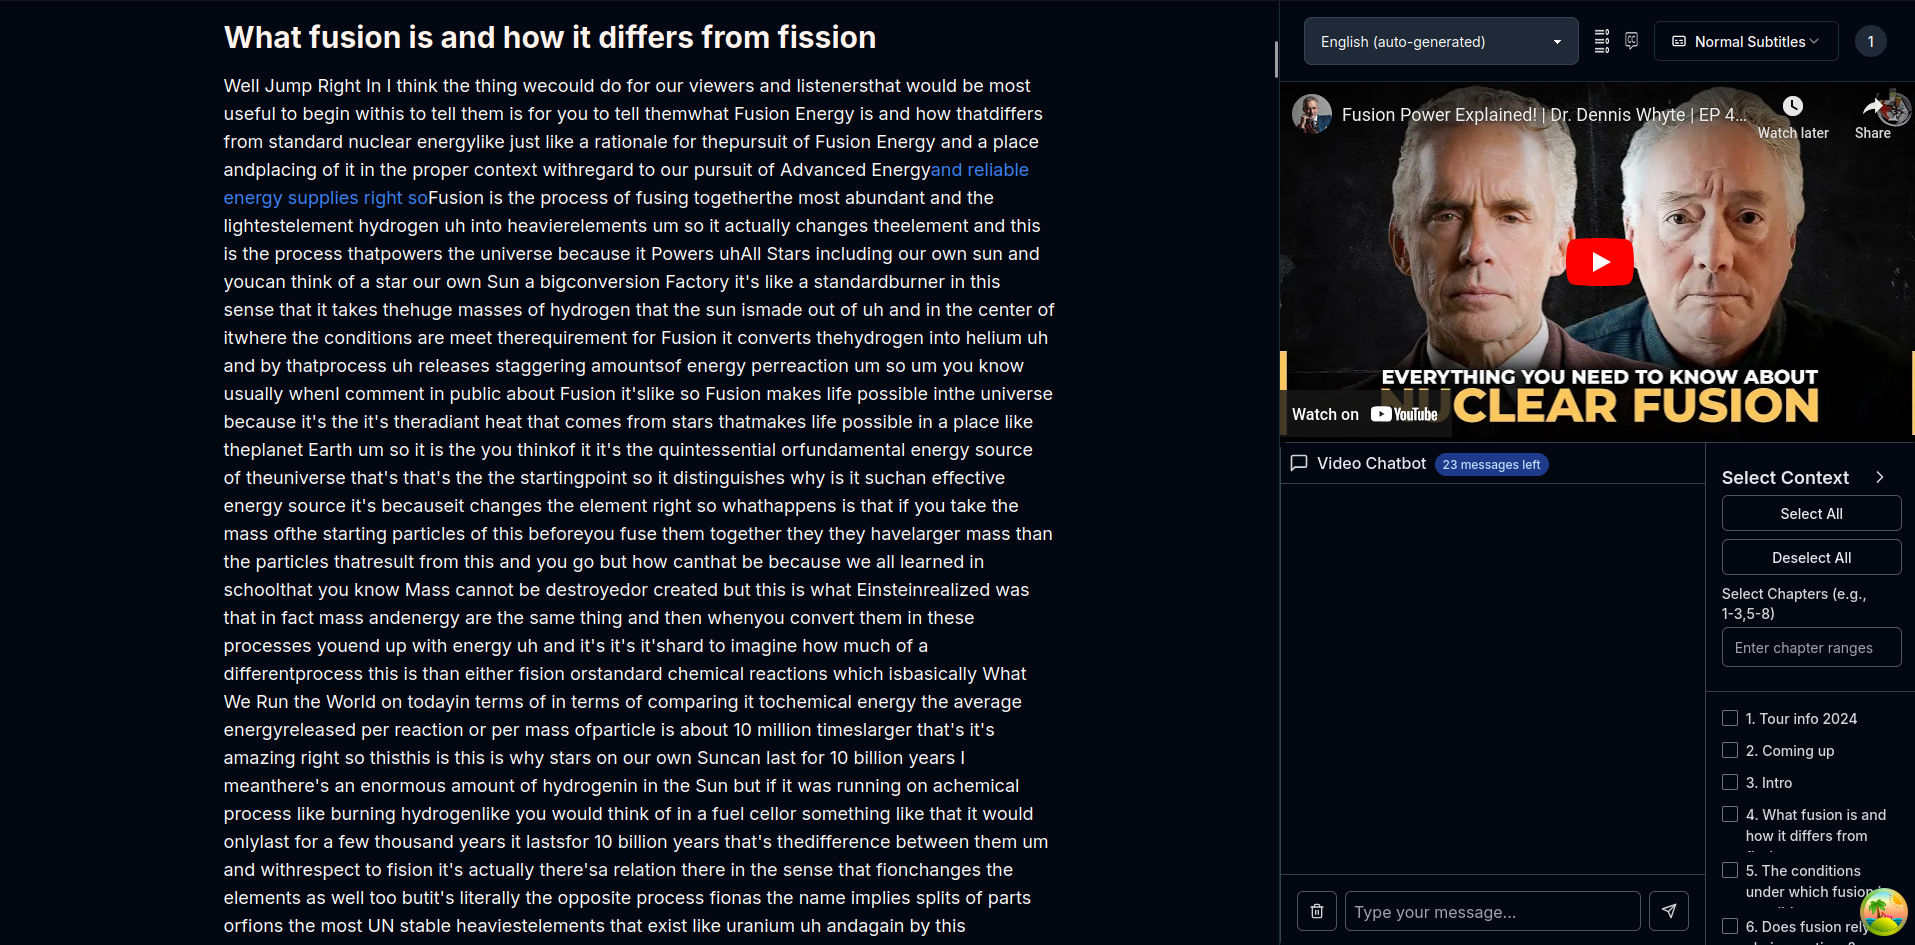
\includegraphics[width=\textwidth,height=\textheight,keepaspectratio]{exemplo-slides/graphics/images/pre-improved-readability.png}
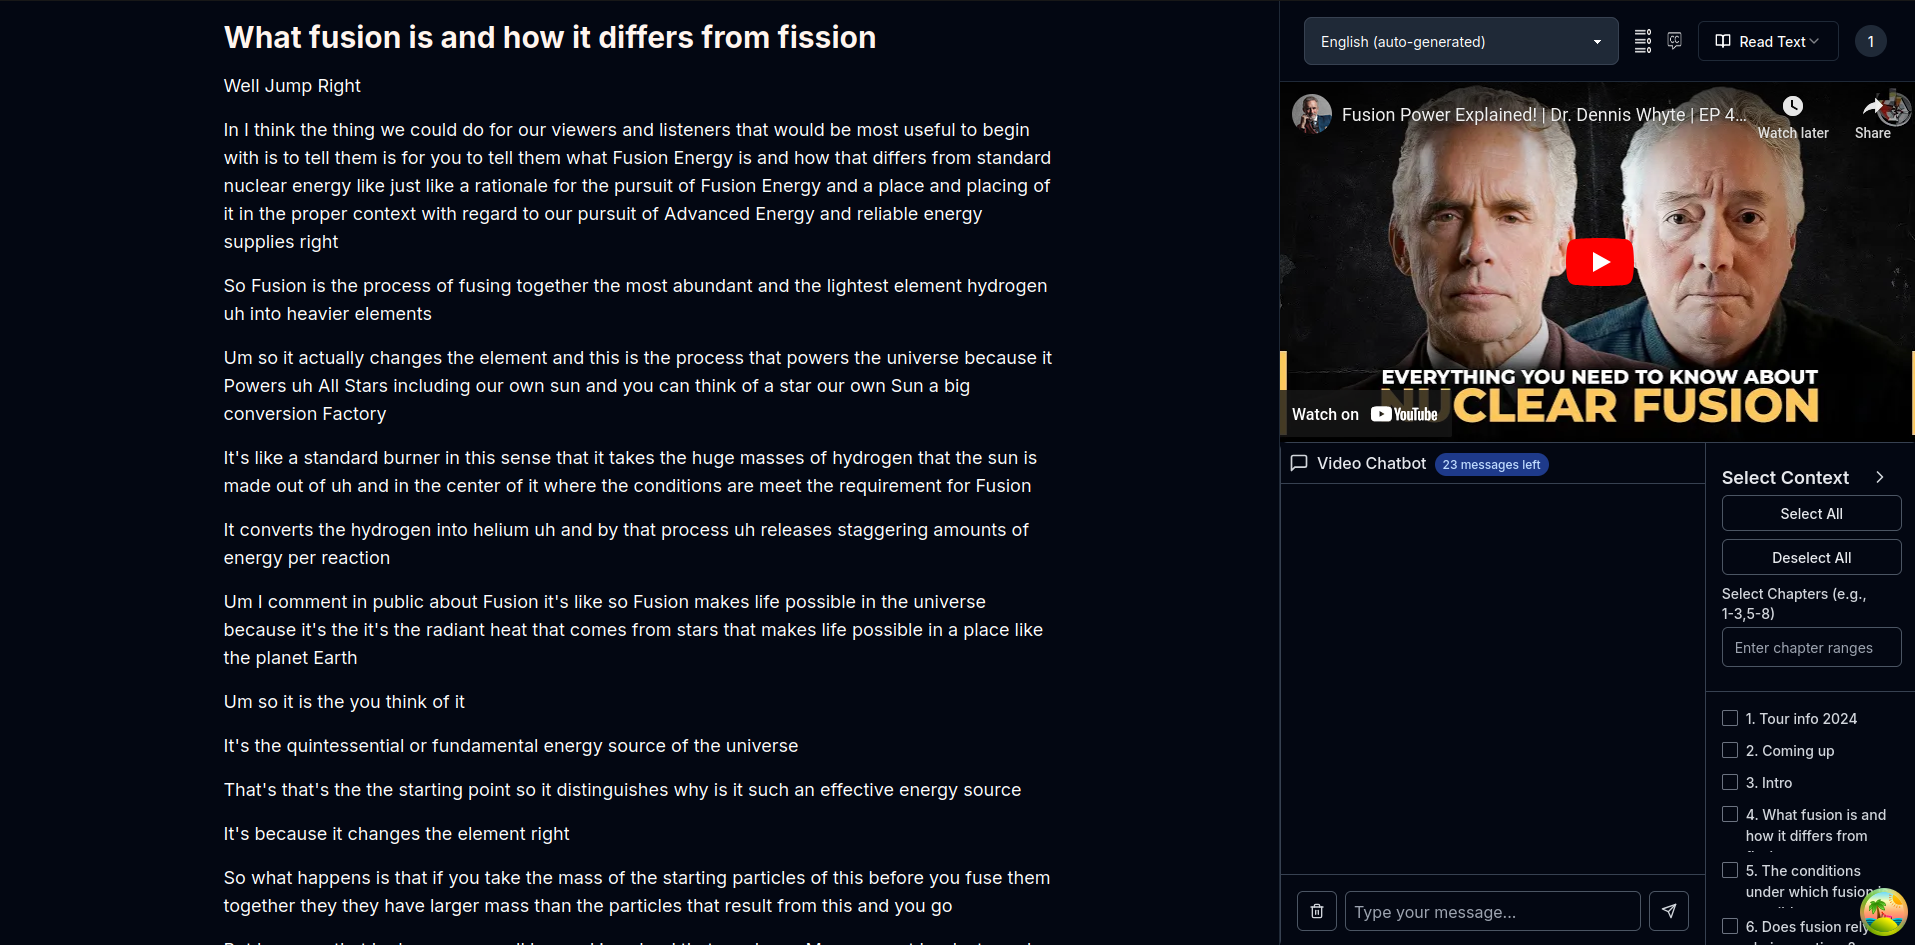
\includegraphics[width=\textwidth,height=\textheight,keepaspectratio]{exemplo-slides/graphics/images/after-improved-readability.png}



\subsection{Comparação e Resultados}
Para avaliar o desempenho das abordagens, foram realizadas comparações entre os textos segmentados pelos LLMs e pelo \texttt{wtpsplit}. Os critérios analisados incluíram:
\begin{itemize}
    \item Tempo de processamento
    \item Fidelidade ao texto original
    \item Legibilidade subjetiva (avaliação qualitativa)
\end{itemize}

Os resultados mostraram que \texttt{wtpsplit} proporcionou uma segmentação mais precisa e eficiente, superando os LLMs em termos de velocidade e fidelidade ao conteúdo original. Assim, a implementação final optou pelo uso de \texttt{wtpsplit} como solução principal para a melhoria da legibilidade das legendas.




\section{Gera\c{c}\~{a}o de Cap\'{i}tulos}

A gera\c{c}\~{a}o autom\'atica de cap\'{i}tulos em v\'{i}deos do YouTube \'{e} um processo essencial para melhorar a navegabilidade e compreens\~{a}o do conte\'udo. Para isso, adotamos um m\'etodo baseado na estrutura\c{c}\~{a}o do texto e na identifica\c{c}\~{a}o de mudan\c{c}as de t\'opico atrav\'es de um modelo de linguagem de grande escala (LLM).

\subsection{Algoritmo e Implementa\c{c}\~{a}o}

O algoritmo segue um fluxo de processamento em tr\^{e}s etapas principais:

1. \textbf{Estrutura\c{c}\~{a}o do texto:} O conte\'udo transcrito do v\'{i}deo \'{e} segmentado em par\'{a}grafos coerentes, respeitando pausas naturais e mudan\c{c}as de contexto no discurso. Essa segmenta\c{c}\~{a}o melhora a compreens\~{a}o e a an\'{a}lise subsequente do texto.

2. \textbf{Numera\c{c}\~{a}o dos par\'{a}grafos:} Cada par\'{a}grafo recebe um identificador num\'erico no in\'{i}cio, o que permite um referenciamento direto na etapa seguinte.

3. \textbf{Identifica\c{c}\~{a}o de mudan\c{c}as de t\'opico:} Utilizamos um LLM para analisar o texto e determinar os par\'{a}grafos que marcam a transi\c{c}\~{a}o entre t\'opicos distintos. O modelo retorna a lista de n\'{u}meros dos par\'{a}grafos que representam pontos de mudan\c{c}a relevantes no conte\'udo.

\subsection{Integra\c{c}\~{a}o com LLMs}

Para a identifica\c{c}\~{a}o das transi\c{c}\~{o}es de t\'opico, utilizamos function calling para interagir com o LLM. Essa abordagem permite enviar a transcri\c{c}\~{a}o segmentada e numerada, solicitando ao modelo que indique os pontos de mudan\c{c}a mais relevantes. A fun\c{c}\~{a}o chamada retorna uma lista de par\'{a}grafos que representam as mudan\c{c}as de t\'opico, possibilitando a gera\c{c}\~{a}o autom\'atica de cap\'{i}tulos estruturados.

Previamente, foi tentado um m\'etodo em que a function calling solicitava apenas o nome dos t\'opicos de transi\c{c}\~{a}o e seu tempo correspondente. No entanto, observou-se um aumento significativo nas alucina\c{c}\~{o}es do modelo. Ao utilizar a numera\c{c}\~{a}o dos par\'{a}grafos, conseguimos reduzir esse problema, pois conhecendo a posi\c{c}\~{a}o do par\'{a}grafo na transcri\c{c}\~{a}o, podemos determinar com maior precis\~{a}o a sua posi\c{c}\~{a}o temporal no v\'{i}deo.

Essa abordagem garante uma segmenta\c{c}\~{a}o eficiente e adapt\'avel, permitindo uma melhor compreens\~{a}o do conte\'udo dos v\'{i}deos e melhorando a experi\^{e}ncia do usu\'ario ao consumir informa\c{c}\~{o}es em formato de v\'{i}deo.





\section{Transcrição}

A transcrição precisa de vídeos do YouTube é essencial para gerar textos mais confiáveis do que as legendas automáticas, que apresentam qualidade inferior especialmente para línguas que não são o inglês.

\subsection{Processo Inicial com Whisper}

No fluxo original utilizando o Whisper, o processo consistia em:

1. \textbf{Download do áudio} (comum a ambos os métodos):
   - Uso da biblioteca \texttt{pytubefix} para download
   - Progresso reportado ao usuário via SSE (Server-Sent Events)
   - Arquivo de áudio com qualidade balanceada entre precisão e velocidade

2. \textbf{Pré-processamento específico para Whisper}:
   - Divisão do áudio em segmentos de 10 minutos
   - Cortes preferencialmente em momentos de silêncio
   - Envio paralelo dos segmentos para transcrição
   - Necessidade decorrente das limitações do Whisper com arquivos longos

\subsection{Migração para o Deepgram}

Com a adoção do Deepgram, o fluxo foi otimizado:

1. \textbf{Download do áudio mantido}:
   - Mesmo processo via \texttt{pytubefix} com feedback via SSE
   - Eliminação da etapa de divisão do áudio

2. \textbf{Transcrição direta}:
   - Envio do arquivo de áudio completo
   - Processamento único sem necessidade de paralelização
   - Interface exibe estimativa de tempo restante
   - Capacidade nativa de lidar com longas durações

\subsection{Comparativo Técnico}

\begin{table}[h]
\centering
\begin{tabular}{|l|c|c|}
\hline
\textbf{Característica} & \textbf{Whisper} & \textbf{Deepgram} \\ \hline
Requer divisão do áudio & Sim & Não \\ \hline
Processamento paralelo & Necessário & Opcional \\ \hline
Feedback em tempo real & Apenas no download & Download + estimativa de transcrição \\ \hline
Limite de duração & 10min/segmento & Até 4h/arquivo \\ \hline
\end{tabular}
\caption{Diferenças na abordagem de transcrição}
\label{tab:abordagem}
\end{table}




\section{Geração de Quizzes}
\subsection{Extração de Conceitos-Chave}
\subsection{Geração via LLM}

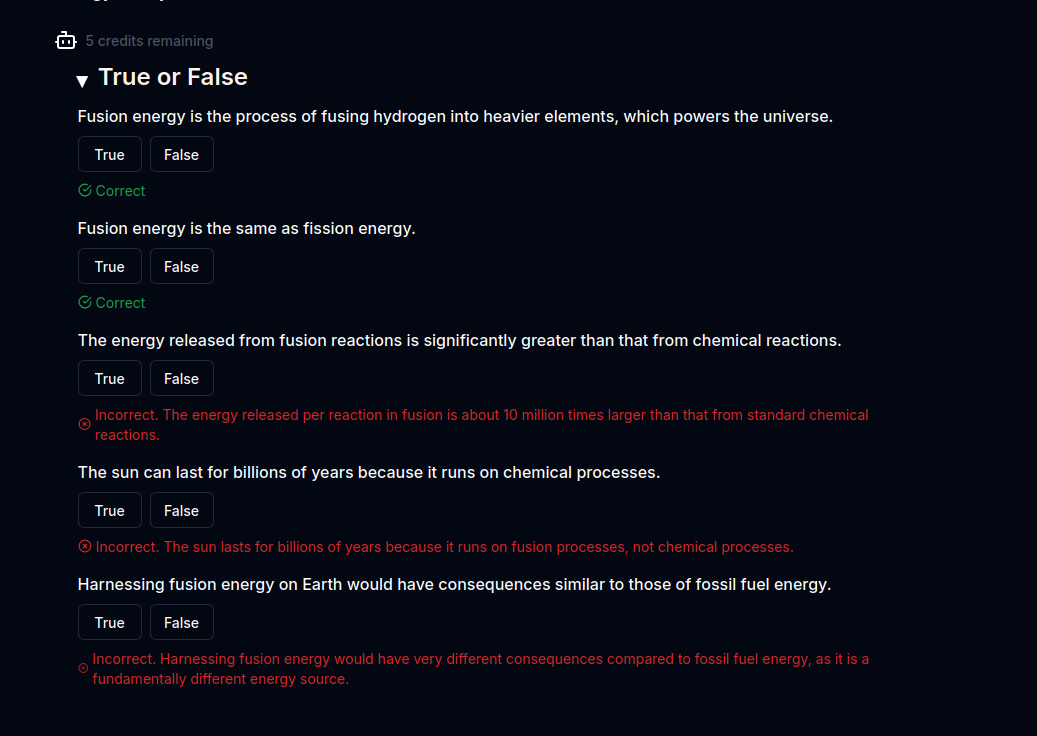
\includegraphics[width=\textwidth,height=\textheight,keepaspectratio]{exemplo-slides/graphics/images/true or false.png}

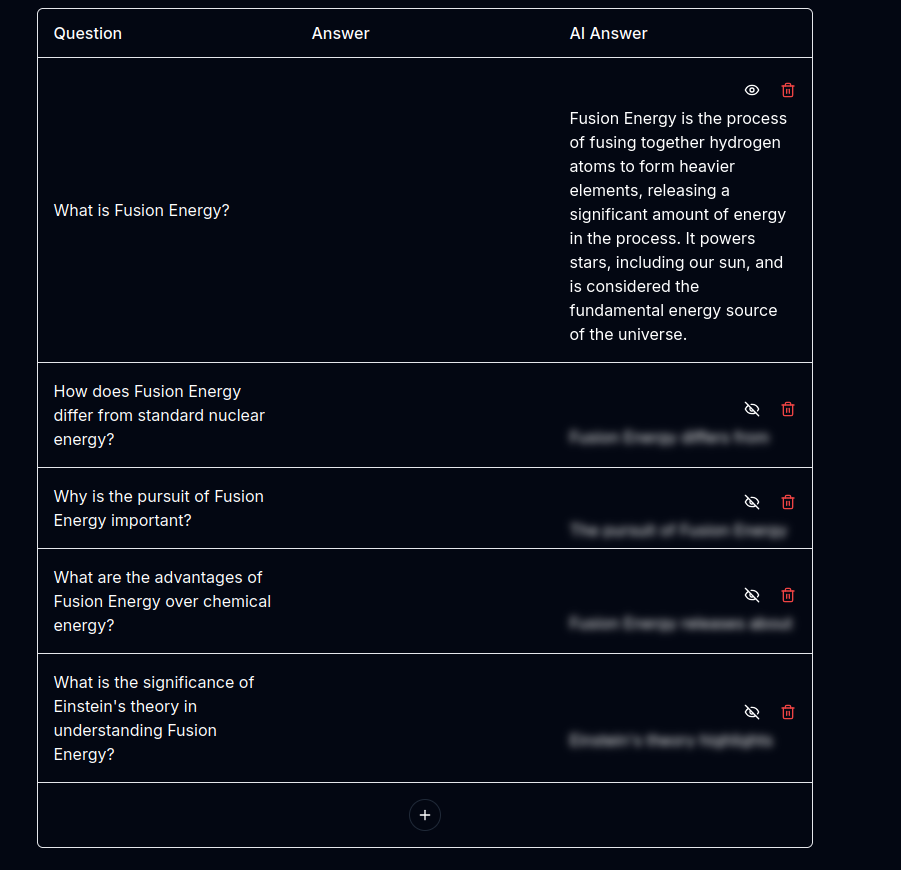
\includegraphics[width=\textwidth,height=\textheight,keepaspectratio]{exemplo-slides/graphics/images/q_a.png}

\section{Bate-Papo com Vídeo}
\subsection{Processamento de Perguntas}
\subsection{Contextualização com Conteúdo}
Durante a interação com o sistema, foi implementada uma funcionalidade que permite ao usuário selecionar capítulos específicos do vídeo que são relevantes para sua pergunta. Esta característica é especialmente importante considerando que, frequentemente, o conteúdo completo do vídeo pode exceder os limites da janela de contexto do modelo de linguagem.

Para garantir uma experiência transparente, o sistema exibe notificações em formato toast quando há risco de exceder a janela de contexto. Embora seja possível selecionar a legenda completa do vídeo, o usuário é alertado quando parte do conteúdo precisa ser truncada devido às limitações técnicas.

A geração de capítulos tornou-se um elemento fundamental neste processo, pois permite que o usuário faça uma seleção precisa do conteúdo pertinente à sua questão, otimizando assim a qualidade das respostas e o uso do contexto disponível.

Em perspectivas futuras, considera-se desenvolver uma abordagem mais agêntica, onde a própria LLM seria responsável por identificar e selecionar os capítulos relevantes para cada pergunta específica. No entanto, nesta primeira implementação, optou-se por manter o controle da seleção nas mãos do usuário.
\subsection{Geração de Respostas}

\section{Desafios e Soluções}
\subsection{Obtenção dos dados do youtube}
\subsection{Utilização de GPU's em produção}


\chapter{Resultados}
\section{Análise de Desempenho}
\section{Feedback dos Usuários}

\chapter{Conclusão}
\section{Objetivos Alcançados}
\section{Trabalhos Futuros}

\chapter{Referências}


% Bibliografia http://liinwww.ira.uka.de/bibliography/index.html um
% site que cataloga no formato bibtex a bibliografia em computacao
% \bibliography{nomedoarquivo.bib} (sem extensao)
% \bibliographystyle{formato.bst} (sem extensao)

\bibliographystyle{abnt}
\bibliography{bibliografia} 

% Apêndices (Opcional) - Material produzido pelo autor
\apendices
\chapter{Um Apêndice}

% Anexos (Opcional) - Material produzido por outro
\anexos
\chapter{Um Anexo}

Bla blabla blablabla bla.  Bla blabla blablabla bla.  Bla blabla
blablabla bla.  Bla blabla blablabla bla.  Bla blabla blablabla bla.
Bla blabla blablabla bla.  Bla blabla blablabla bla.  Bla blabla
blablabla bla.  Bla blabla blablabla bla.  Bla blabla blablabla bla.
Bla blabla blablabla bla.  Bla blabla blablabla bla.  Bla blabla
blablabla bla.  Bla blabla blablabla bla.  Bla blabla blablabla bla.
Bla blabla blablabla bla.  Bla blabla blablabla bla.  Bla blabla
blablabla bla.  Bla blabla blablabla bla.  Bla blabla blablabla bla.
Bla blabla blablabla bla.

Bla blabla blablabla bla.  Bla blabla blablabla bla.  Bla blabla
blablabla bla.  Bla blabla blablabla bla.  Bla blabla blablabla bla.
Bla blabla blablabla bla.  Bla blabla blablabla bla.  Bla blabla
blablabla bla.  Bla blabla blablabla bla.  Bla blabla blablabla bla.
Bla blabla blablabla bla.  Bla blabla blablabla bla.  Bla blabla
blablabla bla.  Bla blabla blablabla bla.  Bla blabla blablabla bla.
Bla blabla blablabla bla.  Bla blabla blablabla bla.  Bla blabla
blablabla bla.  Bla blabla blablabla bla.  Bla blabla blablabla bla.
Bla blabla blablabla bla.

\chapter{Outro Anexo}

Bla blabla blablabla bla.  Bla blabla blablabla bla.  Bla blabla
blablabla bla.  Bla blabla blablabla bla.  Bla blabla blablabla bla.
Bla blabla blablabla bla.  Bla blabla blablabla bla.  Bla blabla
blablabla bla.  Bla blabla blablabla bla.  Bla blabla blablabla bla.
Bla blabla blablabla bla.  Bla blabla blablabla bla.  Bla blabla
blablabla bla.  Bla blabla blablabla bla.  Bla blabla blablabla bla.
Bla blabla blablabla bla.  Bla blabla blablabla bla.  Bla blabla
blablabla bla.  Bla blabla blablabla bla.  Bla blabla blablabla bla.
Bla blabla blablabla bla.

Bla blabla blablabla bla.  Bla blabla blablabla bla.  Bla blabla
blablabla bla.  Bla blabla blablabla bla.  Bla blabla blablabla bla.
Bla blabla blablabla bla.  Bla blabla blablabla bla.  Bla blabla
blablabla bla.  Bla blabla blablabla bla.  Bla blabla blablabla bla.
Bla blabla blablabla bla.  Bla blabla blablabla bla.  Bla blabla
blablabla bla.  Bla blabla blablabla bla.  Bla blabla blablabla bla.
Bla blabla blablabla bla.  Bla blabla blablabla bla.  Bla blabla
blablabla bla.  Bla blabla blablabla bla.  Bla blabla blablabla bla.
Bla blabla blablabla bla.




\end{document}

